
%%%%%%%%%%%%%%%%%%%%%%%%%%%%%%%%%%%%%%%%%%%%%%%%%%%%%%%%%%%%%%%%%%%%%
%% This is a (brief) model paper using the achemso class
%% The document class accepts keyval options, which should include
%% the target journal and optionally the manuscript type.
%%%%%%%%%%%%%%%%%%%%%%%%%%%%%%%%%%%%%%%%%%%%%%%%%%%%%%%%%%%%%%%%%%%%%
\documentclass[journal=jctcce,manuscript=article]{achemso}

%%%%%%%%%%%%%%%%%%%%%%%%%%%%%%%%%%%%%%%%%%%%%%%%%%%%%%%%%%%%%%%%%%%%%
%% Place any additional packages needed here.  Only include packages
%% which are essential, to avoid problems later. Do NOT use any
%% packages which require e-TeX (for example etoolbox): the e-TeX
%% extensions are not currently available on the ACS conversion
%% servers.
%%%%%%%%%%%%%%%%%%%%%%%%%%%%%%%%%%%%%%%%%%%%%%%%%%%%%%%%%%%%%%%%%%%%%
\usepackage[version=3]{mhchem} % Formula subscripts using \ce{}
\usepackage[T1]{fontenc}       % Use modern font encodings
\usepackage{amsmath}	    % American Mathematical Society equation formatting
\graphicspath{ {images/} }     % Path to images

%%%%%%%%%%%%%%%%%%%%%%%%%%%%%%%%%%%%%%%%%%%%%%%%%%%%%%%%%%%%%%%%%%%%%
%% If issues arise when submitting your manuscript, you may want to
%% un-comment the next line.  This provides information on the
%% version of every file you have used.
%%%%%%%%%%%%%%%%%%%%%%%%%%%%%%%%%%%%%%%%%%%%%%%%%%%%%%%%%%%%%%%%%%%%%
%%\listfiles

%%%%%%%%%%%%%%%%%%%%%%%%%%%%%%%%%%%%%%%%%%%%%%%%%%%%%%%%%%%%%%%%%%%%%
%% Place any additional macros here.  Please use \newcommand* where
%% possible, and avoid layout-changing macros (which are not used
%% when typesetting).
%%%%%%%%%%%%%%%%%%%%%%%%%%%%%%%%%%%%%%%%%%%%%%%%%%%%%%%%%%%%%%%%%%%%%
\newcommand*\mycommand[1]{\texttt{\emph{#1}}}

%%%%%%%%%%%%%%%%%%%%%%%%%%%%%%%%%%%%%%%%%%%%%%%%%%%%%%%%%%%%%%%%%%%%%
%% Meta-data block
%% ---------------
%% Each author should be given as a separate \author command.
%%
%% Corresponding authors should have an e-mail given after the author
%% name as an \email command. Phone and fax numbers can be given
%% using \phone and \fax, respectively; this information is optional.
%%
%% The affiliation of authors is given after the authors; each
%% \affiliation command applies to all preceding authors not already
%% assigned an affiliation.
%%
%% The affiliation takes an option argument for the short name.  This
%% will typically be something like "University of Somewhere".
%%
%% The \altaffiliation macro should be used for new address, etc.
%% On the other hand, \alsoaffiliation is used on a per author basis
%% when authors are associated with multiple institutions.
%%%%%%%%%%%%%%%%%%%%%%%%%%%%%%%%%%%%%%%%%%%%%%%%%%%%%%%%%%%%%%%%%%%%%
\author{Alexander Punter}
\author{Paola Nava}
\author{Yannick Carissan}
\email{Yannick.Carissan@univ-amu.fr}
\phone{+33 (0)491289168}
\affiliation[Aix-Marseille University]
{Aix Marseille Univ, CNRS, Centrale Marseille, iSm2, Marseille, France}
%%%%%%%%%%%%%%%%%%%%%%%%%%%%%%%%%%%%%%%%%%%%%%%%%%%%%%%%%%%%%%%%%%%%%
%% The document title should be given as usual. Some journals require
%% a running title from the author: this should be supplied as an
%% optional argument to \title.
%%%%%%%%%%%%%%%%%%%%%%%%%%%%%%%%%%%%%%%%%%%%%%%%%%%%%%%%%%%%%%%%%%%%%
\title[A great title]
  {A great title}

%%%%%%%%%%%%%%%%%%%%%%%%%%%%%%%%%%%%%%%%%%%%%%%%%%%%%%%%%%%%%%%%%%%%%
%% Some journals require a list of abbreviations or keywords to be
%% supplied. These should be set up here, and will be printed after
%% the title and author information, if needed.
%%%%%%%%%%%%%%%%%%%%%%%%%%%%%%%%%%%%%%%%%%%%%%%%%%%%%%%%%%%%%%%%%%%%%
\abbreviations{IR,NMR,UV}
\keywords{Pseudo potentials, Group potentials}

%%%%%%%%%%%%%%%%%%%%%%%%%%%%%%%%%%%%%%%%%%%%%%%%%%%%%%%%%%%%%%%%%%%%%
%% The manuscript does not need to include \maketitle, which is
%% executed automatically.
%%%%%%%%%%%%%%%%%%%%%%%%%%%%%%%%%%%%%%%%%%%%%%%%%%%%%%%%%%%%%%%%%%%%%
\begin{document}

%%%%%%%%%%%%%%%%%%%%%%%%%%%%%%%%%%%%%%%%%%%%%%%%%%%%%%%%%%%%%%%%%%%%%
%% The "tocentry" environment can be used to create an entry for the
%% graphical table of contents. It is given here as some journals
%% require that it is printed as part of the abstract page. It will
%% be automatically moved as appropriate.
%%%%%%%%%%%%%%%%%%%%%%%%%%%%%%%%%%%%%%%%%%%%%%%%%%%%%%%%%%%%%%%%%%%%%
\begin{tocentry}

Some journals require a graphical entry for the Table of Contents.
This should be laid out ``print ready'' so that the sizing of the
text is correct.

Inside the \texttt{tocentry} environment, the font used is Helvetica
8\,pt, as required by \emph{Journal of the American Chemical
Society}.

The surrounding frame is 9\,cm by 3.5\,cm, which is the maximum
permitted for  \emph{Journal of the American Chemical Society}
graphical table of content entries. The box will not resize if the
content is too big: instead it will overflow the edge of the box.

This box and the associated title will always be printed on a
separate page at the end of the document.

\end{tocentry}

%%%%%%%%%%%%%%%%%%%%%%%%%%%%%%%%%%%%%%%%%%%%%%%%%%%%%%%%%%%%%%%%%%%%%
%% The abstract environment will automatically gobble the contents
%% if an abstract is not used by the target journal.
%%%%%%%%%%%%%%%%%%%%%%%%%%%%%%%%%%%%%%%%%%%%%%%%%%%%%%%%%%%%%%%%%%%%%
\begin{abstract}
Very interesting abstract
\end{abstract}

%%%%%%%%%%%%%%%%%%%%%%%%%%%%%%%%%%%%%%%%%%%%%%%%%%%%%%%%%%%%%%%%%%%%%
%% Start the main part of the manuscript here.
%%%%%%%%%%%%%%%%%%%%%%%%%%%%%%%%%%%%%%%%%%%%%%%%%%%%%%%%%%%%%%%%%%%%%
\section{Introduction}

In \cite{Drujon2013}, \ldots .

\section{Method}

\subsection{Making Potentials Physically Meaningful}

So far the method used to obtain the potential parameters has been strictly empirical. We reasoned however that we should be able to make an informed guess at some starting parameters from which to optimise. Clearly the assumption that \(Z = 1\) is unrealistic. The Slater rules suggest that, with the screening effect, the \(p_{z}\) electron should experience a charge of \(Z \approx 2.4\). To mimic the effect of an electron-screened nucleus, we can use a \(p_{z}\) pseudopotential. In order to make an educated guess of the parameters of this new potential, we needed to find an expression for \(Z(\langle r \rangle)\), \( \langle r \rangle \) being the expected distance of the electron from the nucleus. a value we can calculate for orbitals using turbomole parameters.
	The generic forms of Gaussian Type Orbitals for \(s\) and \(p_{z}\) are
\begin{equation}
GTO_{s} = re^{-\alpha r^{2}},\qquad	GTO_{pz} = r \cos \theta e^{-\alpha r^{2}}
\end{equation}
The analytical form of the \(p_{z}\) orbital for a hydrogen-like atom is
\begin{equation}
\phi_{210} = \frac{1}{\sqrt{\pi}} \frac{Z_{eff}}{2a_{0}} ^{\frac{5}{2}} re^{-\frac{z_{eff}r}{2a_{0}}} \cos \theta
\end{equation}
and with the aid of WolframAlpha
\begin{equation}
\langle \phi_{210} | r | \phi_{210} \rangle = \frac{5a_{0}}{Z}
\end{equation}
Next, we need to find a value for \( \langle r \rangle \), which we can extract from our Turbomole calculation

[DERIVATION NEEDED]

Now we can see from (3) that \( \langle r \rangle \approx 1.7\) and therefore that \(Z_{eff} \approx 2.9\). However, the next complication is that this method assumes a complete overlap of the \(p_{z}\) orbital with the \(p_{z}\) pseudopotential which - given that the potential consists only of a single function as compared to the orbital's many - is unlikely to be the case. Therefore we define an overlap matrix \(S\) between \(MO\), the molecular orbital, and \(\chi\), taken from our pseudopotential definition
\begin{equation}
S = \langle MO | \chi \rangle
\end{equation}
where
\begin{equation}
\chi = e^{-\alpha r^{2}},\qquad pp = Z_{pseudo} | \chi \rangle \langle \chi |
\end{equation}
We therefore have
\begin{equation}
\langle \widehat{Z} \rangle = \langle MO | \widehat{Z} | MO \rangle = \langle MO | Z_{pseudo} | \chi \rangle \langle \chi | MO \rangle = Z_{pseudo} S^{2}
\end{equation}
and finally
\begin{equation}
Z_{pseudo} = (Z_{eff} - Z_{nucleus})S^{-2}
\end{equation}

We now have the power to choose a \(p_{z}\) pseudopotential solely based on the Gaussian exponent, and the \(Z_{eff}\) then follows from the above. Clearly, the exponent should be chosen to give us a strong overlap. Hence we arrive at a \(p_{z}\)-potential that should be physically meaningful. 

\subsection{Optimisation}

Optimisations were at first performed of the s and p-potentials to reach the lowest π-orbital energy of ethene. The best set of these potentials was then chosen and the values optimised to match the singlet-triplet energy difference, again of ethene. All optimisations used the Brent method in SciPy's optimisation library, and used standard Hartree-Fock calculations.

\section{Results and discussion}

\begin{table}[ht]
\caption{Reference Values for Relevant Orbital Energies} 
\centering
\begin{tabular}{c c c}
\hline\hline
Calculation Type & CH\(_{3}\)\, \(p_{z}\) energy (eV) & C\(_{2}\)H\(_{4}\)\, \(\pi\) energy (eV) \\
\hline
HF & -10.537 & -10.363 \\
DFT & -6.726 & -6.632 \\
\hline
\end{tabular}
\label{table:ref_values} % is used to refer this table in the text
\end{table}

\begin{table}[ht]
\caption{Optimised s-orbital pseudopotentials for CH\(_{3}\) \((r = 0.5)\)}
\begin{tabular}{c c c}
\hline\hline
Calculation Type & Coefficient & Exponent \\ [0.5ex]
\hline
HF & -2.594 & 1.0 \\
DFT & -2.605 & 1.0 \\
\hline
HF & -4.788 & 5.0 \\
DFT & -4.873 & 5.0 \\
\hline
HF & -7.524 & 10.0 \\
DFT & -7.678 & 10.0 \\
\hline
\end{tabular}
\end{table}

\begin{table}[ht]
\caption{Pseudo-ethene results}
\begin{tabular}{c c c c}
\hline\hline
Calculation Type & \(s\) coefficient & \(s\) exponent & \( \pi \) orbital energy (eV) \\
\hline
\multicolumn{4}{c}{r = 2.0} \\
\hline
HF & -7.521 & 10.0 & -9597 \\
\hline
\multicolumn{4}{c}{r = 0.5} \\
\hline
HF & -7.521 & 10.0 & -7.905 \\
DFT & -7.679 & 10.0 & -8.447 \\
\hline
\end{tabular}
\end{table}

\begin{table}[ht]
\caption{Optimised s-orbital pseudopotentials for CH\(_{3}\)}
\textit{r = 0.5, and \(p_{z}\) potential}
\begin{tabular}{c c c}
\hline\hline
& \(p\) coefficient & \(p\) exponent \\
\hline
\(p_{z}\) potential & -3.267 & 0.295 \\
\hline
Calculation Type & \(s\) coefficient & \(s\) exponent \\
\hline
HF & 2.772 & 1.0 \\
DFT & 3.483 & 1.0 \\
HF & 6.173 & 5.0 \\
DFT & 9.801 & 5.0 \\
HF & 10.381 & 10.0 \\
DFT & 18.351 & 10.0 \\
\hline
\end{tabular}
\end{table}

\begin{table}[ht]
\caption{Pseudo-ethene results}
\textit{default def-SV(P) basis sets, r = 0.5}
\begin{tabular}{c c c c}
\hline\hline
& \(p\) coefficient & \(p\) exponent \\
\hline
\(p_{z}\) potential & -3.267 & 0.295 \\
\hline
Calculation Type & \(s\) coefficient & \(s\) exponent & \(\pi\) orbital energy (eV) \\
\hline
HF & 2.772 & 1.0 & -13.654 \\
DFT & 3.483 & 1.0 & -10.325 \\
HF & 6.173 & 5.0 & -14.011 \\
DFT & 9.801 & 5.0 & -10.409 \\
HF & 10.381 & 10.0 & -14.061 \\
DFT & 18.351 & 10.0 & -12.543 \\
\hline
\end{tabular}
\end{table}

\begin{table}[ht]
\caption{Reference values for ethene excitation energies}
\begin{tabular}{c c c }
\hline\hline
& Energy (H) & Energy (eV) \\
\hline
Singlet & -77.965 \\
Triplet & -77.835 \\
Singlet-Triplet difference & -0.129 & -3.533 \\
Cation & -77.631 \\
Singlet-Cation difference & -0.334 & -9.091 \\
\hline
\end{tabular}
\end{table}

\begin{table}[ht]
\caption{\(s\)-potential fits to ethene \(\pi-\pi*\) excitation}
\begin{tabular}{c c c c c}
\hline\hline
& \(p\) coefficient & \(p\) exponent \\
\hline
\(p_{z}\) potential & -3.267 & 0.295 \\
\hline
s-exponent & s-coefficient & Excitation (eV) & Ionisation (eV) & HOMO energy (eV) \\
\hline 
0.1 & 0.552 & -3.533 & -27.158 & -27.31 \\
1.0 & 0.608 & -3.533 & -28.247 & -28.395 \\
5.0 & 0.936 & -3.533 & -29.583 & -29.722 \\
\hline
\end{tabular}
\end{table}



\begin{figure}
%\includegraphics{properties.jpg}
\caption{\label{fig:properties}%
Comparison of the properties (in eV) obtained with pseudo potentials
and in all electron calculations.}
\end{figure}

\begin{figure}
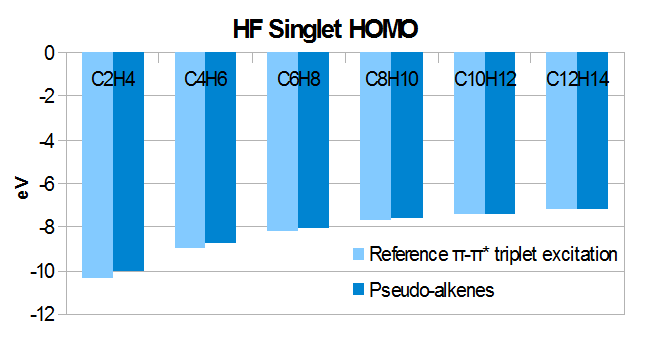
\includegraphics[width=8cm]{hf_homo}
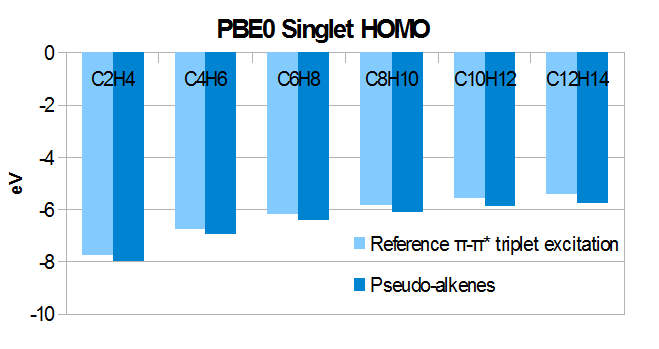
\includegraphics[width=8cm]{pbe0_homo}
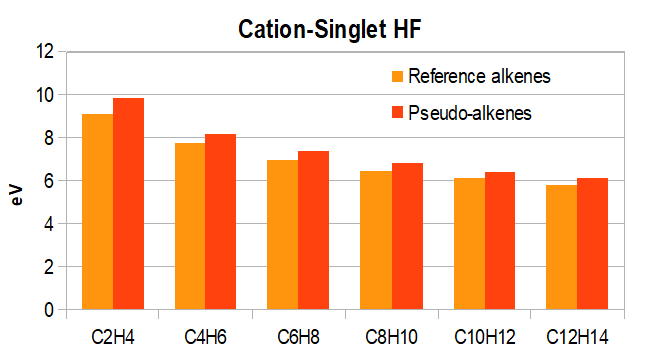
\includegraphics[width=8cm]{hf_ionisation}
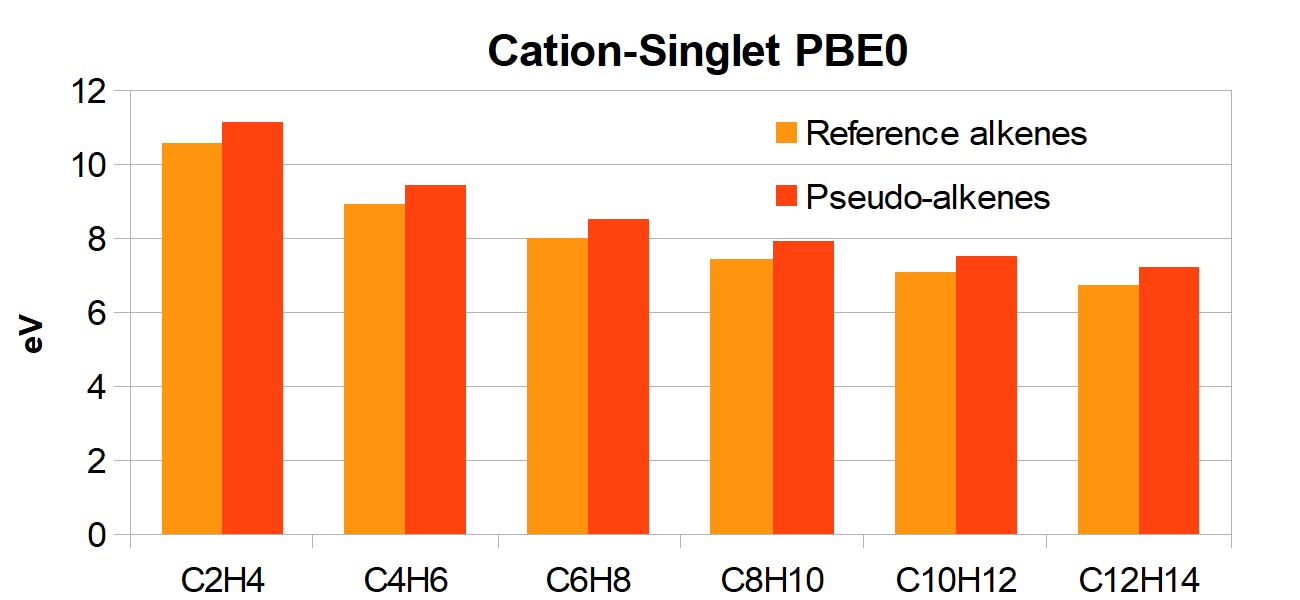
\includegraphics[width=8cm]{pbe0_ionisation}
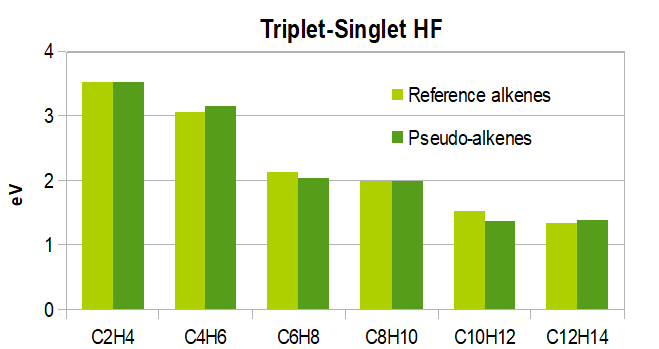
\includegraphics[width=8cm]{hf_excitation}
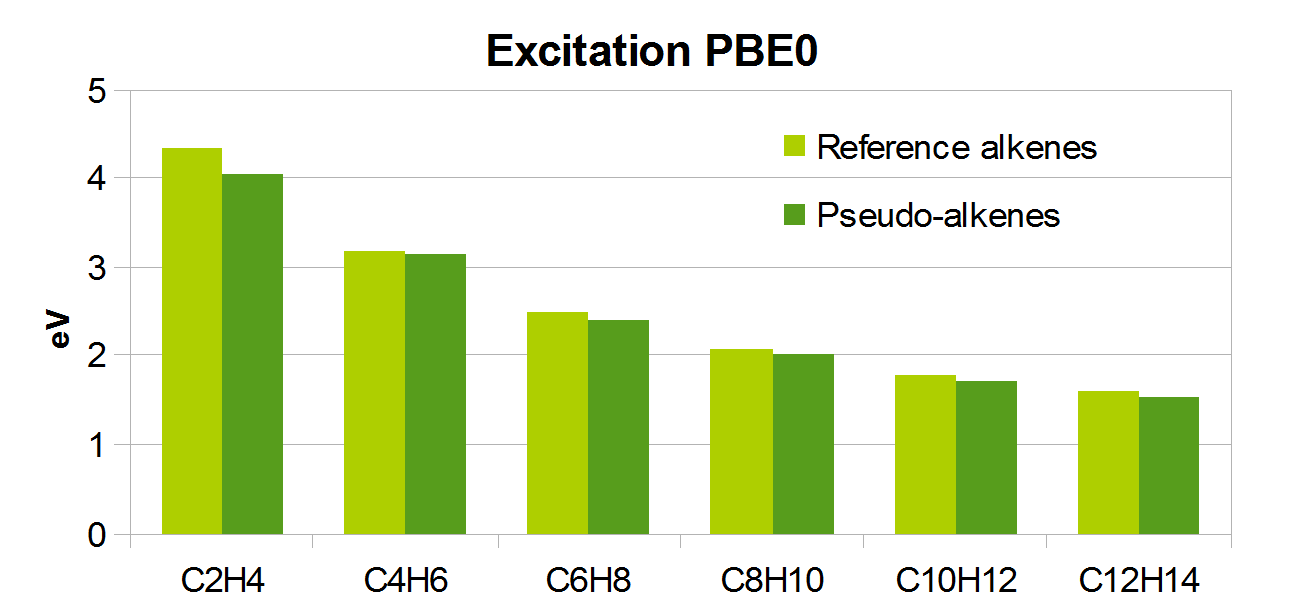
\includegraphics[width=8cm]{pbe0_excitation}
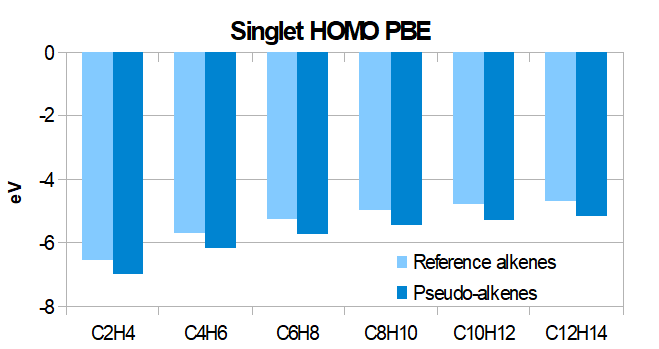
\includegraphics[width=8cm]{pbe_homo}
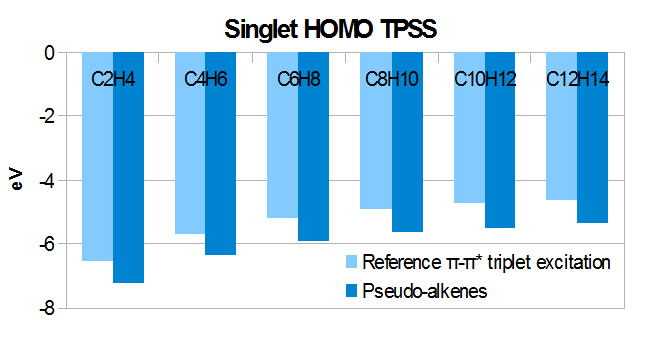
\includegraphics[width=8cm]{tpss_homo}
\end{figure}
\begin{figure}
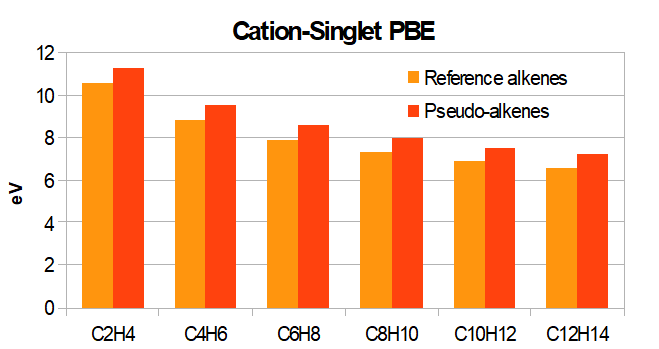
\includegraphics[width=8cm]{pbe_ionisation}
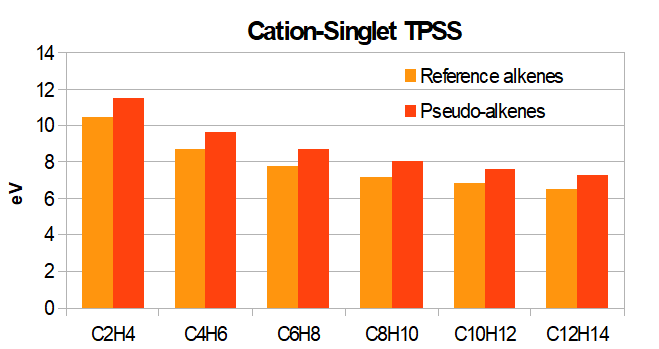
\includegraphics[width=8cm]{tpss_ionisation}
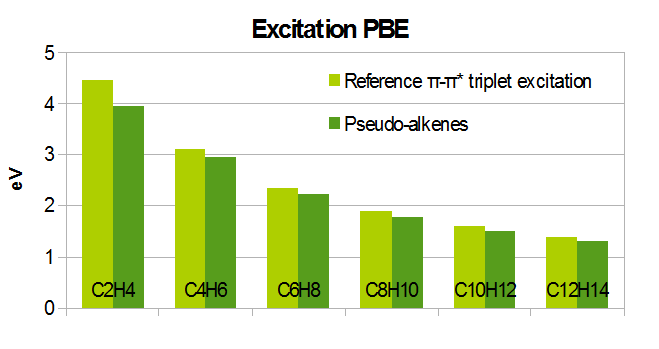
\includegraphics[width=8cm]{pbe_excitation}
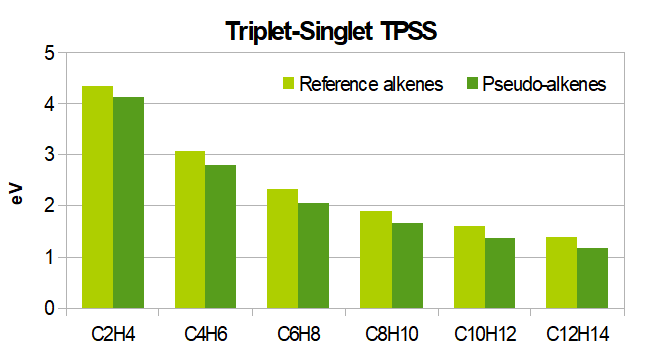
\includegraphics[width=8cm]{tpss_excitation}
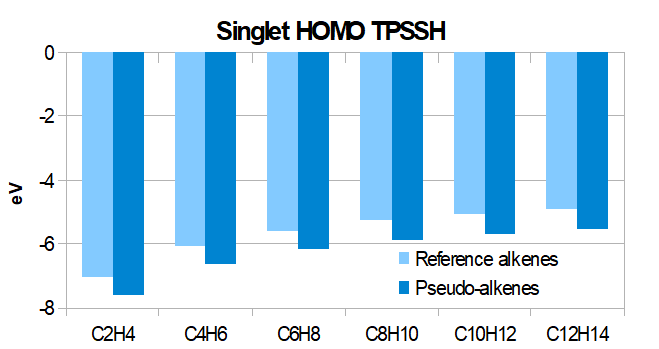
\includegraphics[width=8cm]{tpssh_homo}
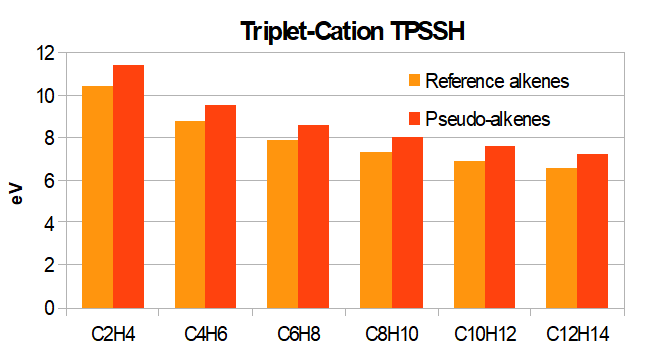
\includegraphics[width=8cm]{tpssh_ionisation}
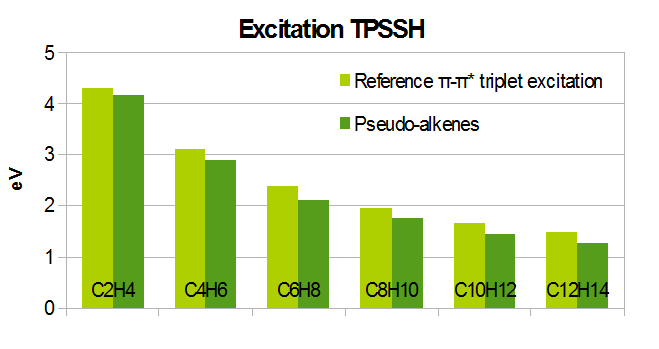
\includegraphics[width=8cm]{tpssh_excitation}
 \caption{\label{fig:hf_excitation}Comparison of reference and pseudosystem energies}
\end{figure}
\begin{figure}
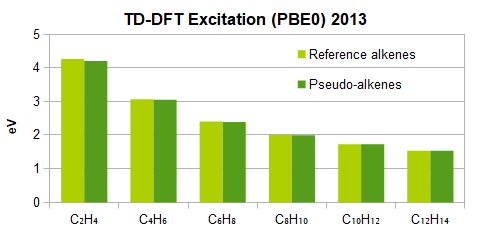
\includegraphics[width=8cm]{tddft_excitation_cd}
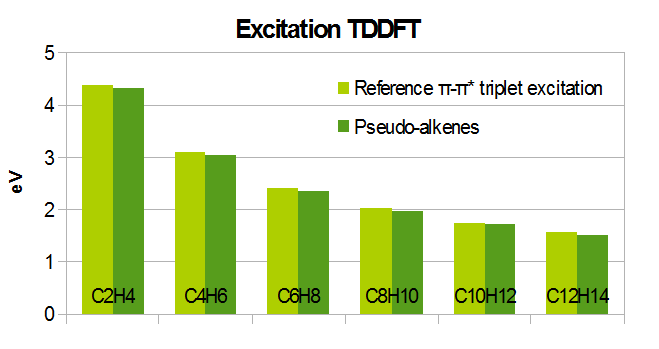
\includegraphics[width=8cm]{tddft_excitation}
 \caption{\label{fig:hf_excitation}Comparison of [CD REF] and new TDDFT calculations}
\end{figure}


%%%%%%%%%%%%%%%%%%%%%%%%%%%%%%%%%%%%%%%%%%%%%%%%%%%%%%%%%%%%%%%%%%%%%
%% The "Acknowledgement" section can be given in all manuscript
%% classes.  This should be given within the "acknowledgement"
%% environment, which will make the correct section or running title.
%%%%%%%%%%%%%%%%%%%%%%%%%%%%%%%%%%%%%%%%%%%%%%%%%%%%%%%%%%%%%%%%%%%%%
\begin{acknowledgement}

The authors thank \ldots

\end{acknowledgement}

%%%%%%%%%%%%%%%%%%%%%%%%%%%%%%%%%%%%%%%%%%%%%%%%%%%%%%%%%%%%%%%%%%%%%
%% The same is true for Supporting Information, which should use the
%% suppinfo environment.
%%%%%%%%%%%%%%%%%%%%%%%%%%%%%%%%%%%%%%%%%%%%%%%%%%%%%%%%%%%%%%%%%%%%%
\begin{suppinfo}

A listing of the contents of each file supplied as Supporting Information
should be included. For instructions on what should be included in the
Supporting Information as well as how to prepare this material for
publications, refer to the journal's Instructions for Authors.

The following files are available free of charge.
\begin{itemize}
  \item Filename: brief description
  \item Filename: brief description
\end{itemize}

\end{suppinfo}

%%%%%%%%%%%%%%%%%%%%%%%%%%%%%%%%%%%%%%%%%%%%%%%%%%%%%%%%%%%%%%%%%%%%%
%% The appropriate \bibliography command should be placed here.
%% Notice that the class file automatically sets \bibliographystyle
%% and also names the section correctly.
%%%%%%%%%%%%%%%%%%%%%%%%%%%%%%%%%%%%%%%%%%%%%%%%%%%%%%%%%%%%%%%%%%%%%
\bibliography{biblio_pseudo_alex}

\end{document}
